\documentclass{standalone}

\usepackage{amsmath}
\usepackage{hyperref}
\usepackage{tikz}
\usepackage{graphicx}

\usetikzlibrary{decorations.pathreplacing,
  arrows,
  calc,
  decorations.pathmorphing,
  decorations.pathreplacing,
  decorations.markings,
  fadings,
  positioning,
  shapes,
  arrows.meta
}
\tikzstyle{snakearrow} = [decorate, decoration={pre length=0.1cm,
  post length=0.1cm, snake, amplitude=.4mm,
  segment length=4mm},thick, ->]
\usepgfmodule{oo}

\pgfdeclareradialshading{glow2}{\pgfpoint{0cm}{0cm}}{
  color(0mm)=(white);
  color(2mm)=(white);
  color(8mm)=(black);
  color(10mm)=(black)
}
\pgfdeclareradialshading{glow}{\pgfpoint{0cm}{0cm}}{
  color(0mm)=(white);
  color(5mm)=(white);
  color(9mm)=(black);
  color(10mm)=(black)
}

\begin{tikzfadingfrompicture}[name=glow fading]
  \shade [shading=glow] (0,0) circle (1);
\end{tikzfadingfrompicture}

\begin{tikzfadingfrompicture}[name=glow2 fading]
  \shade [shading=glow2] (0,0) circle (1);
\end{tikzfadingfrompicture}

\definecolor{atomorange}{rgb}{1.0,0.483,0.0}
\definecolor{pyplotc0}{rgb}{0.122,0.467,0.706}
\definecolor{pyplotc1}{rgb}{1.000,0.498,0.055}
\definecolor{pyplotc2}{rgb}{0.173,0.627,0.173}
\definecolor{pyplotc3}{rgb}{0.839,0.153,0.157}
\definecolor{pyplotc4}{rgb}{0.580,0.404,0.741}
\definecolor{pyplotc5}{rgb}{0.549,0.337,0.294}
\definecolor{pyplotc6}{rgb}{0.890,0.467,0.761}
\definecolor{pyplotc7}{rgb}{0.498,0.498,0.498}
\definecolor{pyplotc8}{rgb}{0.737,0.741,0.133}
\definecolor{pyplotc9}{rgb}{0.090,0.745,0.812}

\pgfdeclarelayer{tweezer}
\pgfsetlayers{tweezer,main}
\pgfooclass{tweezer}{
  \method tweezer() {
  }
  \method drawTweezer(#1,#2,#3) {
    \shade[shading=radial,path fading=glow fading,shift={(#1,#2)},rotate=90,yscale=1,
    fill opacity=0.9,inner color=#3]
    plot[draw,samples=200,domain=-4.5:4.5] function {sqrt(0.02 + (x)**2 / 10)}
    -- plot[draw,samples=200,domain=4.5:-4.5] function {-sqrt(0.02 + (x)**2 / 10)};
  }
  \method drawRaman(#1,#2) {
    \pgfoothis.drawTweezer(#1,#2,pyplotc4);
  }
  \method drawAtom(#1,#2,#3,#4) {
    \fill [#4,path fading=glow2 fading] (#1,#2) circle (#3);
  }
  \method drawDownAtom(#1,#2,#3) {
    \pgfoothis.drawAtom(#1,#2,#3,pyplotc0);
  }
  \method drawUpAtom(#1,#2,#3) {
    \pgfoothis.drawAtom(#1,#2,#3,pyplotc1);
  }
}
\pgfoonew \mytweezer=new tweezer()

\ifpdf
  % Ensure reproducible output
  \pdfinfoomitdate=1
  \pdfsuppressptexinfo=-1
  \pdftrailerid{}
  \hypersetup{
    pdfcreator={},
    pdfproducer={}
  }
\fi

\begin{document}
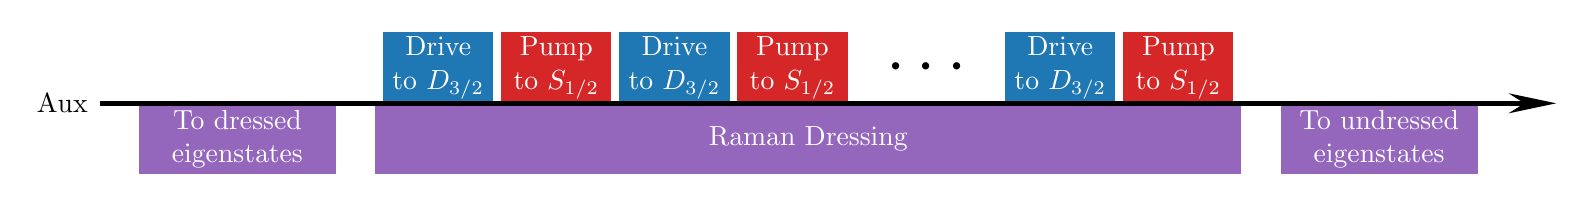
\begin{tikzpicture}
  \begin{scope}[shift={(0, -1.5)}]
    \fill[color=pyplotc4] (-8.5, 0) rectangle (-6, -0.9)
    node[white,pos=.5,align=center] {To dressed\\ eigenstates};

    \fill[color=pyplotc4] (-5.5, 0) rectangle (5.5, -0.9)
    node[white,pos=.5,align=center] {Raman Dressing};

    \fill[color=pyplotc4] (6, 0) rectangle (8.5, -0.9)
    node[white,pos=.5,align=center] {To undressed\\ eigenstates};

    \fill[color=pyplotc0] (-5.4, 0) rectangle (-4, 0.9)
    node[white,pos=.5,align=center] {Drive\\to $D_{3/2}$};
    \fill[color=pyplotc3] (-3.9, 0) rectangle (-2.5, 0.9)
    node[white,pos=.5,align=center] {Pump\\to $S_{1/2}$};

    \fill[color=pyplotc0] (-2.4, 0) rectangle (-1, 0.9)
    node[white,pos=.5,align=center] {Drive\\to $D_{3/2}$};
    \fill[color=pyplotc3] (-0.9, 0) rectangle (0.5, 0.9)
    node[white,pos=.5,align=center] {Pump\\to $S_{1/2}$};

    \node at (1.5, 0.45) {\Huge $\mathbf{\cdots}$};

    \fill[color=pyplotc0] (2.5, 0) rectangle (3.9, 0.9)
    node[white,pos=.5,align=center] {Drive\\to $D_{3/2}$};
    \fill[color=pyplotc3] (4.0, 0) rectangle (5.4, 0.9)
    node[white,pos=.5,align=center] {Pump\\to $S_{1/2}$};

    \draw[-{Stealth[length=6mm,width=2.5mm]},line width=2]
    (-9, 0) node[left] {Aux} -- (9.5, 0);
  \end{scope}
\end{tikzpicture}
\end{document}
